\documentclass{scrartcl}
\usepackage[T1]{fontenc}
\usepackage[utf8]{inputenc}
\usepackage[ngerman]{babel}
\usepackage{amsmath,amssymb}
\usepackage{enumerate}
\usepackage{graphicx}

\begin{document}
\section*{Lösungen zum Thema Graphen}
\begin{enumerate}[(1)]

\item Knoten $1,2,3,4$ und folgende Kanten mit Gewichten: $c(\{1,2\})=1$, $c(\{2,3\})=1$, $c(\{3,4\})=1$ und $c({1,4})=2$.
Bilde den k\"urzeste-Wege-Baum von $1$ aus. Benutzte Kanten: $\{1,2\}, \{2,3\}, \{1,4\}$ mit Gewicht 4.
Der minimale Spannbaum besteht aus den drei Kanten mit Gewicht 1 (Gesamtgewicht 3).

\item \begin{enumerate}[(a)]
\item Knoten $1,2,3$ und folgende Kanten mit Gewichten: $c(\{1,2\})=3$, $c(\{2,3\})=-2$, und $c(\{1,3\})=2$. Startknoten sei Knoten $1$.
\item Knoten $1,2,3$ und folgende Kanten mit Gewichten: $c(\{1,2\})=1$, $c(\{2,3\})=-1$, und $c(\{1,3\})=9$. Startknoten sei wieder Knoten $1$.
\item bei ungerichteten Graphen gilt: negative Kante = negativer Kreis (Kante beliebig oft vor und zur\"uck).
\end{enumerate}

\item \begin{enumerate}[(a)]
	\item \ \\ 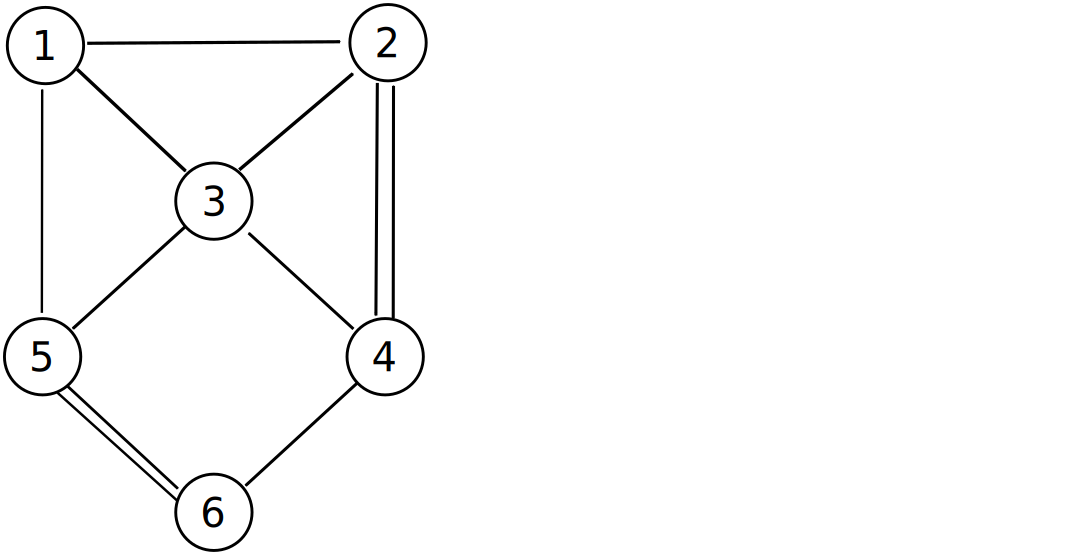
\includegraphics[width=5cm]{images/Graphdarstellungsaufgabe}
	\item \ \\ 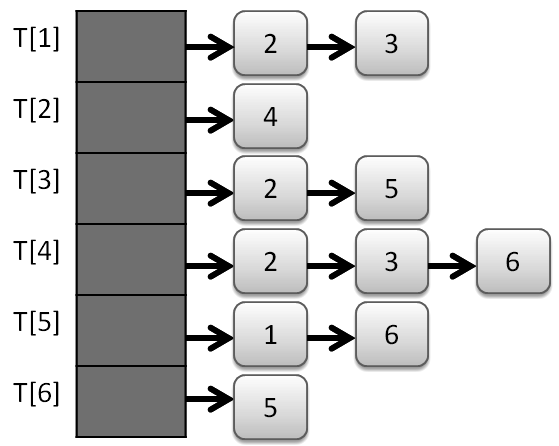
\includegraphics[width=6cm]{images/AdjazenzlisteSW}
	\item Die dritte vorgestellte Möglichkeit ist die Adjazenzmatrixdarstellung. In einer $|V| \times |V|$-Matrix $A$ wird an der Stelle $A_{i,j}$ eine 1 gesetzt, wenn zwischen den Knoten i und j eine Kante existiert, andernfalls eine 0.\\
	Vorteile:
	\begin{itemize}
		\item Problem ''Existiert Kante von i nach j?'' in konstanter Zeit lösbar
		\item Einfaches Hinzufügen und Löschen von Kanten möglich
		\item manche Graphenoperationen direkt durch Matrixoperationen durchführbar (z.B. ''Existiert ein Pfad von A nach B?'' durch Potenzieren der Adjazenzmatrix)
	\end{itemize}
	Nachteile:
	\begin{itemize}
		\item verhältnismäßig hoher Speicherverbrauch bei dünnen Graphen
	\end{itemize}
\end{enumerate}
\end{enumerate}
\end{document}